\subsection{\texorpdfstring{\(\tau\)-扩张的直像}{\textbackslash tau-扩张的直像}}

设 G 是一个群，设 F 与 \(F'\) 是交换群，设 \(\tau\)（相应地，\(\tau'\)）是一个群同态（从 G 到 F（相应地，\(F'\)）的自同构群的），并设 \(v: F \to F'\) 是一个群同态，使得

\[
v (\tau (g) \cdot f) = \tau^ {\prime} (g) \cdot v (f)\tag{3}
\]

（对每个 \(g \in G\) 与 \(f \in F\)）。设 \(\mathcal{E} = (\Gamma, \iota, \pi)\) 是 G 被 F 的一个 \(\tau\)-扩张。设 \(\widetilde{\Gamma}\) 是外半直积 \(F' \times_{\tau' \circ \pi} \Gamma\)。用 \(\widetilde{\iota}: F' \to \widetilde{\Gamma}\) 表示同态 \(f \mapsto (f, e)\)，并用 \(\widetilde{p}: \widetilde{\Gamma} \to \Gamma\) 表示第一个投影。设 \(j: F \to \widetilde{\Gamma}\) 是由 \(f \mapsto (v(f), \iota(f)^{-1})\) 定义的映射。由于 \(\iota\) 的像包含在 \(\tau' \circ \pi\) 的核中，映射 j 是一个群同态；由于 \(\iota\) 是单射的，它是单射的。我们有关系

\[
\begin{array}{r l} (f ^ {\prime}, \gamma) j (f) (f ^ {\prime}, \gamma) ^ {- 1} & = (f ^ {\prime}, \gamma) (v (f), \iota (f) ^ {- 1}) (f ^ {\prime}, \gamma) ^ {- 1} \\ & = (\tau^ {\prime} (\pi (\gamma)) \cdot v (f), \iota (\tau (\pi (\gamma)) \cdot f) ^ {- 1}) \\ & = j (\tau (\pi (\gamma)) \cdot f) \end{array}\tag{4}
\]

（对 \(f \in F\)、\(\gamma \in \Gamma\) 与 \(f' \in F'\)）。因此，j 的像是 \(\widetilde{\Gamma}\) 的一个正规子群。用 \(\Gamma'\) 表示 \(\widetilde{\Gamma}\) 关于 j 的像的商。用 \(\iota'\) 表示从 \(\widetilde{\Gamma}\) 到 \(\Gamma'\) 的典范满射与 \(\widetilde{\iota}\) 的复合。同态 \(\pi \circ \widetilde{p}\) 的核是积 \(\mathrm{F}' \times \iota(\mathrm{F})\)，它包含 j 的像。我们把 \(\pi' : \Gamma' \to G\) 定义为由 \(\pi \circ \widetilde{p}\) 通过过渡到商得到的群同态。由于 \(\iota\) 是单射的，\(j(\mathrm{F})\) 与 \(\widetilde{\iota}(\mathrm{F}')\) 的交化归为 \(\widetilde{\Gamma}\) 的单位元素；由此推出 \(\iota'\) 是单射的。从 \(F' \times F\) 到 \(F' \times \iota(\mathrm{F}) = \operatorname{Ker}(\pi \circ \widetilde{p})\) 的由

\[
(f ^ {\prime}, f) \longmapsto (f ^ {\prime} v (f), \iota (f) ^ {- 1})
\]

给出的映射是一个群同构。于是 \(\iota'\) 的像与 \(\pi'\) 的核重合。由于 \(\pi\) 与 \(\widetilde{p}\) 是满射的，\(\pi'\) 也是满射的。这就证明了 \(\mathcal{E}' = (\Gamma', \iota, \pi')\) 是一个 \(\tau'\)-扩张（\(G\) 被 \(F'\) 的）；我们称它为 \(\mathcal{E}\) 被 \(v\) 的直像，并记作 \(v_{*}(\mathcal{E})\)。从 \(\widetilde{\Gamma}\) 到 \(\Gamma'\) 的典范满射与从 \(\Gamma\) 到 \(\widetilde{\Gamma}\) 的由 \(\gamma \mapsto (1, \gamma)\) 给出的群同态的复合是一个群同态 \(\varphi : \Gamma \to \Gamma'\)，我们称之为典范的。

命题 2. —— 用上面的记号，下面的图交换：

\begin{enumerate}
\def\labelenumi{(\arabic{enumi})}
\setcounter{enumi}{4}
\tightlist
\item
\end{enumerate}

\pandocbounded{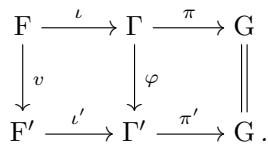
\includegraphics[keepaspectratio]{images/part002_f3abcdb3.jpg}}

设 \(\mathcal{E}_1' = (\Gamma_1', \iota_1', \pi_1')\) 是一个 \(\tau'\)-扩张（G 被 F' 的），并设 \(\varphi_1: \Gamma \to \Gamma_1'\) 是一个使得下图交换的群同态：

\pandocbounded{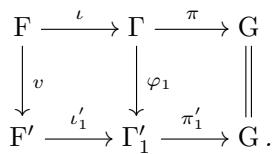
\includegraphics[keepaspectratio]{images/part002_c84edb93.jpg}}

则存在唯一的态射 \(\psi\)（\(\tau'\)-扩张的、从 \(v_{*}(\mathcal{E})\) 到 \(\mathcal{E}_1'\) 的），使得我们有 \(\varphi_1 = \psi \circ \varphi\)。

第一个图的交换性由构造得出。\(\psi\) 的存在性与唯一性由下面的引理 3 得出。

引理 3. —— 设 \(G_{1}^{\prime}\) 是一个群，并设 \(w: G \to G_{1}^{\prime}\) 与 \(\tau_{1}: G_{1}^{\prime} \to \operatorname{Aut}(F^{\prime})\) 是满足 \(\tau^{\prime} = \tau_{1} \circ w\) 的群同态。设 \(\mathcal{E}_{1}^{\prime} = (\Gamma_{1}^{\prime}, \iota_{1}^{\prime}, \pi_{1}^{\prime})\) 是一个 \(\tau_{1}\)-扩张（\(G_{1}^{\prime}\) 被 \(F^{\prime}\) 的），并设 \(\varphi_{1}: \Gamma \to \Gamma_{1}^{\prime}\) 是一个使得下图交换的群同态：

\[
\begin{array}{c} \mathrm{F} \xrightarrow {\iota} \Gamma \xrightarrow {\pi} \mathrm{G} \\ \Biggl \downarrow_ {v} \qquad \qquad \Biggl \downarrow_ {\varphi_ {1}} \qquad \Biggl \downarrow_ {w} \\ \mathrm{F} ^ {\prime} \xrightarrow {\iota_ {1} ^ {\prime}} \Gamma_ {1} ^ {\prime} \xrightarrow {\pi_ {1} ^ {\prime}} \mathrm{G} _ {1} ^ {\prime}. \end{array}
\]

则存在唯一的群同态 \(\psi : \Gamma' \to \Gamma'_1\)，使得图

\[
\begin{array}{c} \mathrm{F} ^ {\prime} \xrightarrow {\iota^ {\prime}} \Gamma^ {\prime} \xrightarrow {\pi^ {\prime}} \mathrm{G} \\ \Big \| \qquad \qquad \qquad \Big \downarrow_ {\psi} \qquad \Big \downarrow_ {w} \\ \mathrm{F} ^ {\prime} \xrightarrow {\iota_ {1} ^ {\prime}} \Gamma_ {1} ^ {\prime} \xrightarrow {\pi_ {1} ^ {\prime}} \mathrm{G} _ {1} ^ {\prime} \end{array}
\]

交换且 \(\varphi_{1} = \psi \circ \varphi\)。

对任何 \((f,\gamma)\in\mathrm{F}^{\prime}\times\Gamma\)，把 \((f,\gamma)\) 在 \(\Gamma^{\prime}\) 中的类记作 \(\overline{(f,\gamma)}\)。若群同态 \(\psi:\Gamma^{\prime}\to\Gamma_{1}^{\prime}\) 具有所要的性质，则它满足关系

\[
\psi \big (\overline {{(f ^ {\prime} , \gamma)}} \big) = \psi (\iota^ {\prime} (f ^ {\prime}) \varphi (\gamma)) = \iota_ {1} ^ {\prime} (f ^ {\prime}) \varphi_ {1} (\gamma)
\]

（对每个 \(f' \in \mathrm{F}'\) 与 \(\gamma \in \Gamma\)）。反之，映射 \(\tilde{\psi}\) 从 \(\mathrm{F}' \times_{\tau' \circ \pi} \Gamma\) 到 \(\Gamma_1'\) 由 \((f, \gamma) \mapsto \iota_1'(f) \varphi_1(\gamma)\) 给出，是一个群同态。实际上，我们有关系

\[
\begin{array}{r} \iota_ {1} ^ {\prime} (f) \varphi_ {1} (\gamma) \iota_ {1} ^ {\prime} (f ^ {\prime}) \varphi_ {1} (\gamma^ {\prime}) = \iota_ {1} ^ {\prime} (f \tau_ {1} (\pi_ {1} ^ {\prime} (\varphi_ {1} (\gamma))) \cdot f ^ {\prime}) \varphi_ {1} (\gamma \gamma^ {\prime}) \\ = \iota_ {1} ^ {\prime} (f \tau^ {\prime} (\pi (\gamma)) \cdot f ^ {\prime}) \varphi_ {1} (\gamma \gamma^ {\prime}) \end{array}
\]

（对 \(f, f' \in \mathrm{F}'\) 与 \(\gamma, \gamma' \in \Gamma\)）。\(\widetilde{\psi}\) 的核包含 \(j\) 的像，因为 \(\iota_1'(v(f)) = \varphi_1(\iota(f))\)（对 \(f \in \mathrm{F}\)），而态射 \(\psi\)（由 \(\widetilde{\psi}\) 通过过渡到商得到的）具有所要的性质。

注. —— 用 \(\Sigma\) 表示 \(\tau'\)-扩张的结构种，并把 \(\alpha\)-映射定义为从 \(\Gamma\) 到群 \(\Gamma'\)（某一个 \(\tau'\)-扩张的底层群）的映射，它们是群同态且使下图交换：

\[
\begin{array}{c} \mathrm{F} \xrightarrow {\iota} \Gamma \xrightarrow {\pi} \mathrm{G} \\ \Big \downarrow v \qquad \qquad \Big \downarrow \varphi \\ \mathrm{F} ^ {\prime} \xrightarrow {\iota^ {\prime}} \Gamma^ {\prime} \xrightarrow {\pi^ {\prime}} \mathrm{G}. \end{array}\tag{6}
\]

命题 2 表示 \(v_{*}(\mathcal{E})\) 是相应的普遍映射问题的一个解（集合论, IV, §3, No.~1, 第 284 页）。

推论 1. —— 设 \(E_{1}\) 与 \(E_{2}\) 是 G 被 F 的 \(\tau\)-扩张，并设 \(\psi\) 是一个 \(\tau\)-扩张的态射（从 \(E_{1}\) 到 \(E_{2}\) 的）。用 \(\varphi_{1}\)（相应地，\(\varphi_{2}\)）表示 \(v_{*}(\mathcal{E}_{1})\)（相应地，\(v_{*}(\mathcal{E}_{2})\)）的典范同态。则存在唯一的 \(\tau'\)-扩张的态射（从 \(v_{*}(\mathcal{E}_{1})\) 到 \(v_{*}(\mathcal{E}_{2})\) 的），记作 \(v_{*}(\psi)\)，使得 \(\varphi_{2} \circ \psi = v_{*}(\psi) \circ \varphi_{1}\)。

只需对 \(\varphi_{2} \circ \psi\) 应用命题 2。

于是 \(\tau^{\prime}\)-扩张 \(v_{*}(\mathcal{E})\) 的类只依赖于 E 的类。我们也用 \(v_{*}:\operatorname{Ex}_{\tau}(\mathrm{G},\mathrm{F})\to\operatorname{Ex}_{\tau^{\prime}}(\mathrm{G},\mathrm{F}^{\prime})\) 表示把一个 \(\tau\)-扩张 E 的类映到 \(\tau^{\prime}\)-扩张 \(v_{*}(\mathcal{E})\) 的类的映射。

推论 2. —— 我们保留命题的记号。设 F'' 是一个交换群，并设 \(\tau'' : G \to \text{Aut}(F'')\) 与 \(v': F' \to F''\) 是满足

\[
\tau^ {\prime \prime} (g) \cdot v ^ {\prime} (f) = v ^ {\prime} (\tau^ {\prime} (g) \cdot f)
\]

（对 \(g \in G\) 与 \(f \in F'\)）的群同态。设 E 是 G 被 F 的一个 \(\tau\)-扩张，并用 \(\varphi\)（相应地，\(\varphi'\)、\(\varphi''\)）表示与 \(v_{*}(\mathcal{E})\)（相应地，\(v_{*}'(v_{*}(\mathcal{E}))\)、\((v' \circ v)_{*}(\mathcal{E})\)）相伴的典范同态。则存在唯一的态射 \(\psi\)（从 \(\tau''\)-扩张 \(v_{*}'(v_{*}(\mathcal{E}))\)（G 被 \(F''\) 的）到 \(\tau''\)-扩张 \((v' \circ v)_{*}(\mathcal{E})\) 的），使得 \(\varphi'' = \psi \circ \varphi' \circ \varphi\)。

例. —— 1) 设 \(j: \{1\} \to \mathrm{F}\) 是典范单射。半平凡扩张 \(\mathcal{I}_{\tau}\) 同构于 \(j_{*}((\mathrm{G}, i, \mathrm{Id}_{\mathrm{G}}))\)，其中 \(i: \{e\} \to \mathrm{G}\) 是典范单射。设 \(c: \mathrm{F} \to \mathrm{F}\) 是常值同态 \(f \mapsto 1\)，并设 \(\mathcal{E}\) 是一个 \(\tau\)-扩张。\(\tau\)-扩张 \(c_{*}(\mathcal{E})\) 也同构于 \(\mathcal{I}_{\tau}\)。

\begin{enumerate}
\def\labelenumi{\arabic{enumi})}
\setcounter{enumi}{1}
\tightlist
\item
  设 E 是 F 的一个在 G 的作用下稳定的子群。用 \(F'\) 表示 F 模 E 的商，用 \(v : F \to F'\) 表示典范同态，并用 \(\tau' : G \to \text{Aut}(F')\) 表示 G 在 \(F'\) 上的作用，它由
\end{enumerate}

\[
\tau^ {\prime} (g) \cdot v (f) = v (\tau (g) \cdot f)
\]

（对 \(g \in G\) 与 \(f \in F\)）刻画。设 \(\mathcal{E} = (\Gamma, \iota, \pi)\) 是 G 被 F 的一个 \(\tau\)-扩张。则 \(\iota(\mathrm{E})\) 是 \(\Gamma\) 的一个正规子群，且 \(\tau'\)-扩张 \(v_{*}(\mathcal{E})\)（G 被 \(F'\) 的）同构于扩张 \((\Gamma/\iota(\mathrm{E}), \bar{\iota}, \overline{\pi})\)，其中 \(\bar{\iota}\) 与 \(\overline{\pi}\) 是由 \(\iota\) 与 \(\pi\) 通过过渡到商得到的群同态。借助这个同构，典范同态 \(\varphi\)（与 \(v_{*}(\mathcal{E})\) 相伴的）对应于从 \(\Gamma\) 到 \(\Gamma/\iota(\mathrm{E})\) 的典范同态。

命题 3. —— 设 G 与 G' 是群，并设 F 与 F' 是交换群。设 \(\tau: \mathrm{G} \to \mathrm{Aut}(\mathrm{F})\)、\(\tau': \mathrm{G} \to \mathrm{Aut}(\mathrm{F}')\)、\(u: \mathrm{G}' \to \mathrm{G}\) 与 \(v: \mathrm{F} \to \mathrm{F}'\) 是满足

\[
\tau^ {\prime} (g) \cdot v (f) = v (\tau (g) \cdot f)
\]

（对 \(g \in G\) 与 \(f \in F\)）的群同态。我们记 \(\tau'' = \tau' \circ u\)。设 E 是 G 被 F 的一个 \(\tau\)-扩张。我们用 \(\varphi_u\)（相应地，\(\varphi_v\)、\(\varphi'_u\)、\(\varphi'_v\)）表示对应于 \(\tau \circ u\)-扩张 \(u^*(\mathcal{E})\)（相应地，\(\tau'\)-扩张 \(v_*(\mathcal{E})\)、\(\tau''\)-扩张 \(u^*(v_*(\mathcal{E}))\) 与 \(v_*(u^*(\mathcal{E})))\)）的典范同态。则存在唯一的态射 \(\psi\)（\(\tau''\)-扩张的，从 \(v_*(u^*(\mathcal{E}))\) 到 \(u^*(v_*(\mathcal{E}))\)），使得 \(\varphi_v \circ \varphi_u = \varphi'_u \circ \psi \circ \varphi'_v\)。

我们把 \(\tau \circ u\)-扩张 \(u^{*}(\mathcal{E})\)（相应地，\(\tau''\)-扩张 \(u^{*}(v_{*}(\mathcal{E}))\)）记作 \((\Gamma_u, \iota_u, \pi_u)\)（相应地，\((\Gamma_u', \iota_u', \pi_u')\)）。把 VIII, 第 287 页的引理 2 应用于 \(\varphi_v \circ \varphi_u\)，我们得到存在一个群同态 \(\psi_{1}:\Gamma_{u}\to\Gamma_{u}^{\prime}\)，使得图

\pandocbounded{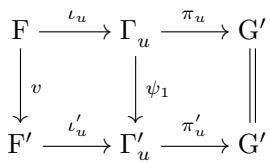
\includegraphics[keepaspectratio]{images/part002_ccea47d6.jpg}}

交换且 \(\varphi_{u}^{\prime}\circ\psi_{1}=\varphi_{v}\circ\varphi_{u}\)。\(\psi\) 的存在性由应用于 \(\psi_{1}\) 的命题 2 得出。反之，若 \(\psi^{\prime}\) 也具有所要的性质，则由引理 2 我们有 \(\psi^{\prime}\circ\varphi_{v}^{\prime}=\psi_{1}\)，故 \(\psi^{\prime}=\psi\)（命题 2）。

